% !TeX document-id = {efee450f-6069-4a1d-a54f-d3ae0eb7270d}
% !TeX TXS-program:compile = txs:///pdflatex/[-shell-escape]

\documentclass[11pt]{beamer}
\usepackage[utf8]{inputenc}
\usepackage[T1,T2A]{fontenc}
\usepackage[russian]{babel}
\usepackage{color}
\usepackage{calc}
\usepackage{graphicx}
\usepackage{epstopdf}
\usepackage{hyperref}
\hypersetup{unicode,colorlinks}
\usetheme[progressbar=head,numbering=fraction,block=fill]{metropolis}
\usepackage{minted}
\usepackage{dejavu}
%\usepackage{adjustbox}  % Позволяет сузить куски кода (или текст) ровно настолько, чтобы уместиться в слайд
\usepackage{csquotes}
\usepackage{upquote}

\usemintedstyle{solarized-light}
\newminted[haskell]{haskell}{
    escapeinside=!!,
    mathescape=true,
    texcomments=true,
    beameroverlays=true,
    autogobble=true,
    fontsize=\small,
    breaklines=false  % Лучше сам поставлю переносы на удобных местах
}
\newminted[haskellsmall]{haskell}{
    escapeinside=!!,
    mathescape=true,
    texcomments=true,
    beameroverlays=true,
    autogobble=true,
    fontsize=\footnotesize,
    breaklines=false
}
\newminted[haskelltiny]{haskell}{
    escapeinside=!!,
    mathescape=true,
    texcomments=true,
    beameroverlays=true,
    autogobble=true,
    fontsize=\scriptsize,
    breaklines=false
}
\newmintinline[haskinline]{haskell}{
    escapeinside=!!,
    mathescape=true,
    beameroverlays=true,
    breaklines=true
}
\newminted[ghci]{text}{
    autogobble=true,
    fontsize=\small,
    breaklines=false
}
\newminted[ghcismall]{text}{
    autogobble=true,
    fontsize=\footnotesize,
    breaklines=false
}
\newminted[ghcitiny]{text}{
    autogobble=true,
    fontsize=\scriptsize,
    breaklines=false
}
\newmintinline[ghcinline]{text}{
    breaklines=true
}

\newcommand{\hackage}[1]{\href{https://hackage.haskell.org/package/#1}{#1}}

\vfuzz=20pt  % позволяет тексту дойти до номера слайда

\author{Алексей Романов}
\subtitle{Функциональное программирование на Haskell}
%\logo{}
\institute{МИЭТ}
\subject{Функциональное программирование на Haskell}
%\setbeamercovered{transparent}
%\setbeamertemplate{navigation symbols}{}


\title{Лекция 13: многопоточность}

\begin{document}
\begin{frame}[plain]
  \maketitle
\end{frame}

\begin{frame}[fragile]
  \frametitle{Два вида многопоточности: конкурентность и параллелизм}
  \begin{itemize}
    \item Все программы, которые мы писали до сих пор, были однопоточными.
    \item У современных компьютеров много ядер, мы задействуем только одно.
    \item Чтобы использовать их, нужна многопоточность. \pause
    \item Параллелизм: физическая многопоточность. Много ядер (или других ресурсов) используются для ускорения выполнения одной задачи. \pause
    \item Конкурентность: логическая многопоточность. Несколько задач, которые могут выполняться логически одновременно. А значит, потенциально и физически одновременно.
  \end{itemize}
\end{frame}

\begin{frame}[fragile]
  \frametitle{Детерминированность}
  \begin{itemize}
    \item Модель программирования детерминирована, если результат программы зависит только от полученных данных (аргументов и ввода пользователя). \pause
    \item Недетерминирована, если результат зависит от того, в каком порядке произойдут события (или от сгенерированных случайных чисел и т.д.). \pause
    \item Обычно параллельные программы детерминированы, конкурентные нет.
    \item Недетерминированность усложняет тестирование, отладку и понимание программ, но часто без неё не обойтись.
    \item Тестирование свойств это пример пользы от недетерминированности.
  \end{itemize}
\end{frame}

\begin{frame}[fragile]
  \frametitle{Параллелизм: монада \haskinline|Eval|}
  \begin{itemize}
    \item Модуль \haskinline|Concurrent.Parallel.Strategies| в пакете \hackage{parallel}.
    \item Тип \haskinline|Eval a| --- монада, где в \haskinline|mx >>= f| значение \haskinline|mx| будет вычислено до СЗНФ перед запуском \haskinline|f|. \pause
    \item Есть функции
          \begin{haskell}
            runEval :: Eval a -> a
            rpar :: a -> Eval a
            rseq :: a -> Eval a
            parEval :: Eval a -> Eval a
          \end{haskell}
    \item \haskinline|rpar x|: запустить вычисление \haskinline|x| и сразу вернуться.
    \item \haskinline|rseq x|: вернуться после вычисления \haskinline|x|.
    \item \haskinline|parEval x|: запустить вычисление, описанное в \haskinline|x|, и сразу вернуться.
  \end{itemize}
\end{frame}

\begin{frame}[fragile]
  \frametitle{Примеры \haskinline|Eval|}
  \begin{itemize}
    \item
          Запуск двух вычислений параллельно:
          \begin{haskell}
            runEval $ do
              a <- rpar (f x)
              b <- rpar (f y)
              return (a, b)
          \end{haskell}
          %                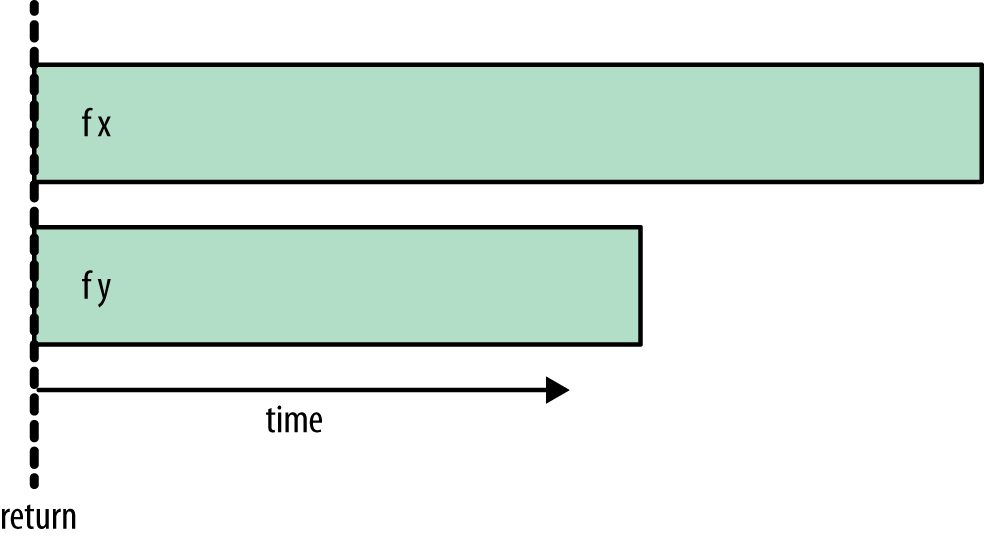
\includegraphics[width=\textwidth]{concurrency_eval1.png}
          \pause
    \item
          Запуск двух вычислений параллельно и возврат, когда оба закончатся:
          \begin{haskell}
            runEval $ do
              a <- rpar (f x)
              b <- rseq (f y)
              rseq a
              return (a, b)
          \end{haskell}
          %    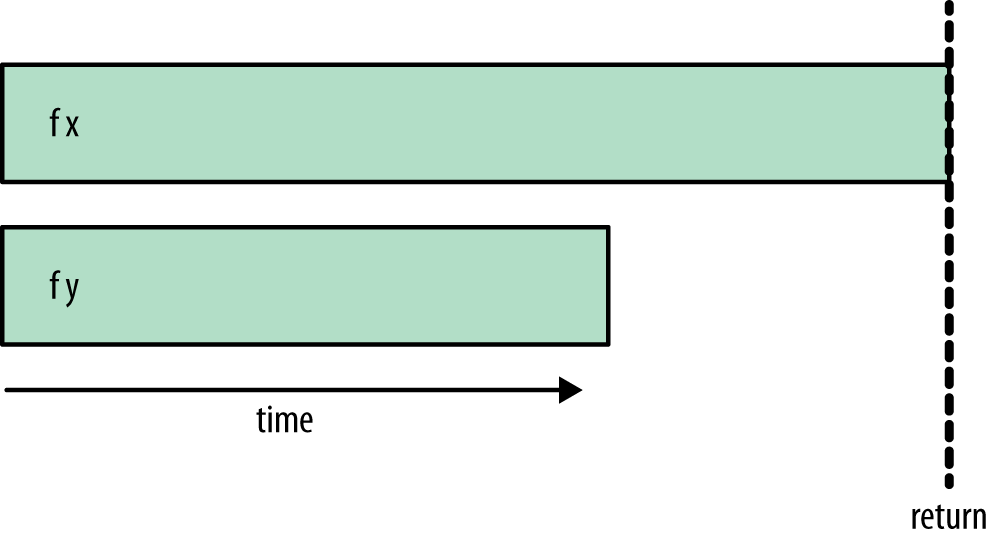
\includegraphics[width=\textwidth]{concurrency_eval2.png}
  \end{itemize}
\end{frame}

\begin{frame}[fragile]
  \frametitle{Фибоначчи в \haskinline|Eval|}
  \begin{itemize}
    \item
          \begin{haskellsmall}
            parFib1 :: Integer -> Integer
            parFib1 0 = 1
            parFib1 1 = 1
            parFib1 n = runEval $ do !\pause!
              f1 <- rpar (parFib1 (n - 1))
              f2 <- rseq (parFib1 (n - 2))
              -- rseq, чтобы занять текущий поток, можно и rpar
              pure (f1 + f2)
          \end{haskellsmall}
          \pause
    \item
          \begin{haskellsmall}
            parFib2 :: Integer -> Eval Integer
            parFib2 0 = pure 1
            parFib2 1 = pure 1
            parFib2 n = do !\pause!
              f1 <- parEval (parFib2 (n - 1))
              f2 <- parFib2 (n - 2)
              pure (f1 + f2)
          \end{haskellsmall}
          \pause
    \item Здесь для простоты кода много повторных вычислений!
  \end{itemize}
\end{frame}

% TODO восстановить слайд
%\begin{frame}[fragile]
%\frametitle{Примеры \haskinline|Eval|}
%\begin{columns}
%    \begin{column}{0.5\textwidth}
%        Запуск двух вычислений параллельно:
%\begin{haskell}
%runEval $ do
%  a <- rpar (f x)
%  b <- rpar (f y)
%  return (a, b)
%\end{haskell}
%%    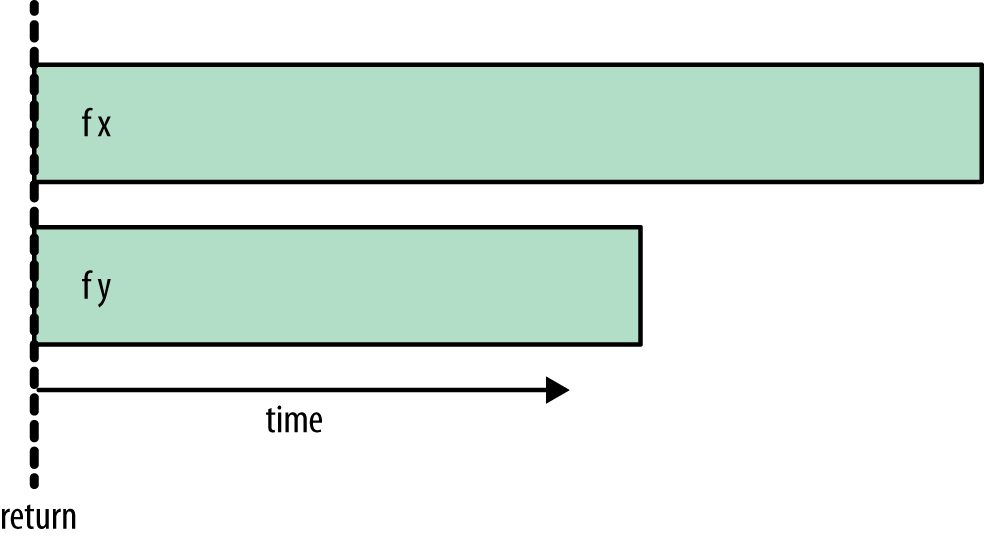
\includegraphics[width=\textwidth]{concurrency_eval1.png}
%    \end{column}\pause
%    \begin{column}{0.5\textwidth}
%    Запуск двух вычислений параллельно и возврат, когда оба закончатся:
%\begin{haskell}
%runEval $ do
%  a <- rpar (f x)
%  b <- rseq (f y)
%  rseq a
%  return (a, b)
%\end{haskell}
%%    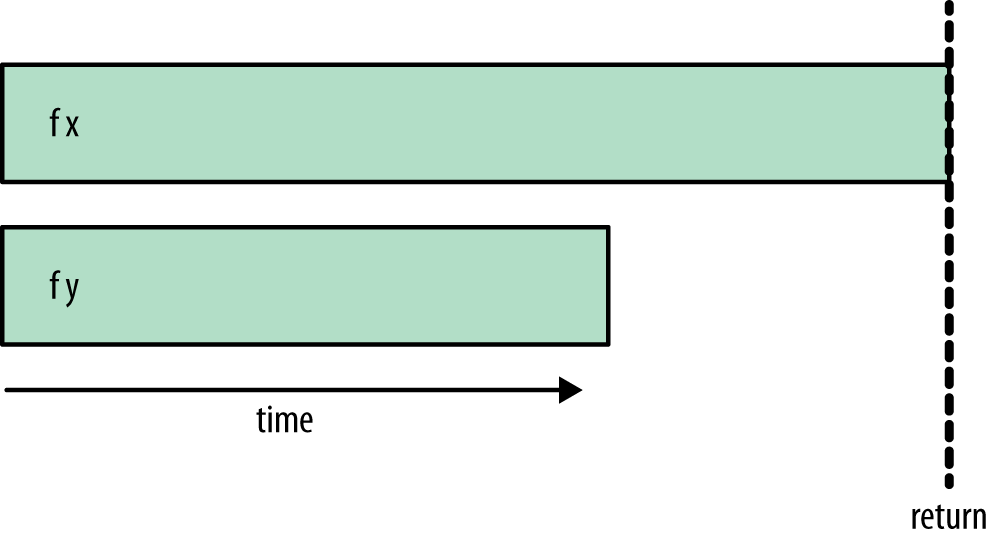
\includegraphics[width=\textwidth]{concurrency_eval2.png}
%    \end{column}
%\end{columns}
%\end{frame}

\begin{frame}[fragile]
  \frametitle{Стратегии вычислений}
  \begin{itemize}
    \item \haskinline|type Strategy a = a -> Eval a|.
    \item \haskinline|rpar| и \haskinline|rseq| --- стратегии.
    \item \haskinline|r0| --- стратегия, которая ничего не вычисляет.
    \item Стратегия принимает на вход thunk, вычисляет его части с помощью \haskinline|r0|, \haskinline|rpar| и \haskinline|rseq|.
    \item Например, обобщая пример с прошлого слайда
          \begin{haskell}
            rparTuple2 :: Strategy (a, b)
            rparTuple2 (a, b) = do !\pause!
              a' <- rpar a
              b' <- rpar b
              return (a', b')
          \end{haskell}
          \pause
          (или \haskinline[fontsize=\small]|rparTuple2 (a, b) = liftA2 (,) (rpar a) (rpar b)|)
    \item
          \begin{haskell}
withStrategy :: Strategy a -> a -> a
withStrategy s x = runEval (s x)
\end{haskell}
  \end{itemize}
\end{frame}

\begin{frame}[fragile]
  \frametitle{Комбинаторы стратегий}
  \begin{itemize}
    \item Обобщим \haskinline|rparTuple2| дальше, чтобы она принимала стратегии на вход:
          \begin{haskell}
            evalTuple2 :: Strategy a -> Strategy b -> 
              Strategy (a, b)
            evalTuple2 strat_a strat_b (a, b) = !\pause! 
              liftA2 (,) (strat_a a) (strat_b b)
          \end{haskell}
          \pause
    \item \haskinline|rparWith :: Strategy a -> Strategy a| запускает стратегию параллельно.
    \item Например, \haskinline|rparWith rpar| и \haskinline|rparWith rseq| эквивалентны \haskinline|rpar|.
          \pause
    \item
          \begin{haskell}
            parTuple2 :: Strategy a -> Strategy b -> 
              Strategy (a, b)
            parTuple2 strat_a strat_b = 
              evalTuple2 (rparWith strat_a) (rparWith strat_b)
          \end{haskell}
  \end{itemize}
\end{frame}

\begin{frame}[fragile]
  \frametitle{Комбинаторы стратегий для списков}
  \begin{itemize}
    \item С помощью стратегий достаточно легко сделать параллельные \haskinline|map|/\haskinline|filter|/и т.д.
    \item Например, используя \haskinline|parList :: Strategy a -> Strategy [a]|:
          \begin{haskell}
            parallelMap :: (a -> b) -> [a] -> [b]
            parallelMap f xs = 
              withStrategy (parList rseq) (map f xs)
          \end{haskell}
          \pause
    \item Это скорее всего создаст слишком много \enquote{искр}, лучше использовать
          \begin{itemize}
            \item \haskinline|parListChunk|: разбивает список на части одинаковой длины и работает параллельно с каждой частью
            \item \haskinline|parBuffer|: начинает работать параллельно с первыми элементами списка, добавляет следующие при использовании результатов
          \end{itemize}
  \end{itemize}
\end{frame}

\begin{frame}[fragile]
  \frametitle{Монада \haskinline|Par|: параллелизм без ленивости}
  \begin{itemize}
    \item Модуль \haskinline|Control.Monad.Par| в пакете \haskinline|monad-par|.
    \item Тип \haskinline|Par a| --- тоже монада, описывающая процесс вычисления значения типа \haskinline|a| с параллельными частями.
    \item \haskinline|fork :: Par () -> Par ()| создаёт новый поток.
    \item \haskinline|runPar :: Par a -> a| производит вычисление и возвращает его результат. \pause
    \item Потоки общаются между собой с помощью \haskinline|IVar|, которые можно записать только 1 раз.
    \item В результате не должно быть \haskinline|IVar| или ссылок на них!
    \item При соблюдении этого условия вычисления в \haskinline|Par| детерминированы.
  \end{itemize}
\end{frame}

\begin{frame}[fragile]
  \frametitle{\haskinline|IVar|}
  \begin{itemize}
    \item Интерфейс \haskinline|IVar|:
          \begin{haskell}
            new :: Par (IVar a)
            newFull :: NFData a => a -> Par (IVar a)
            put :: NFData a => IVar a -> a -> Par ()
            get :: IVar a -> Par a
          \end{haskell}
    \item Значения, положенные в \haskinline|IVar|, полностью вычисляются (есть ещё \haskinline|newFull_| и \haskinline|put_|).
    \item Переменной можно дать значение только 1 раз, иначе исключение.
    \item При вызове \haskinline|get| для переменной, ещё не имеющей значения, начинается ожидание.
  \end{itemize}
\end{frame}

\begin{frame}[fragile]
  \frametitle{Примеры \haskinline|Par|}
  \begin{itemize}
    \item \haskinline|spawn :: NFData a => Par a -> Par (IVar a)|: аналог \haskinline|fork|, но возвращающий переменную, в которой будет сохранено вычисленное значение
          \begin{haskell}
            spawn par = do
              var <- new
              fork $ do (x <- par; put var x)
              return var
          \end{haskell}
    \item Параллельный \haskinline|map|:
          \begin{haskell}
            parallelMap :: NFData b => (a -> b) -> [a] -> [b]
            parallelMap f xs = runPar $ do
              ivars <- mapM (spawn (\x -> pure (f x)) xs
              mapM get ivars
          \end{haskell}
          Как и в прошлый раз, создаёт \enquote{поток} для каждого элемента, для простоты кода.
  \end{itemize}
\end{frame}

\begin{frame}[fragile]
  \frametitle{Фибоначчи в \haskinline|Par|}
  \begin{itemize}
    \begin{haskell}
      parFib :: Integer -> Par Integer
      parFib 0 = pure 1
      parFib 1 = pure 1
      parFib n = do !\pause!
        f1var <- spawn (parFib (n - 1))
        f2 <- parFib (n - 2)
        f1 <- get f1var
        pure (f1 + f2)
    \end{haskell}
  \end{itemize}
\end{frame}

\begin{frame}[fragile]
  \frametitle{Конкурентность}
  \begin{itemize}
    \item Перейдём от параллелизма к конкурентности.
    \item Модуль \haskinline|Control.Concurrent| в пакете \haskinline|base| и \haskinline|C.C.MVar|/\haskinline|C.C.Chan|/\haskinline|C.C.QSem[N]|.
    \item \haskinline|ThreadId| --- ссылка на поток.
    \item \haskinline|forkIO :: IO () -> IO ThreadId| создаёт новый поток, который произведёт данные действия и выйдет, возвращает ссылку на созданный поток.
          \pause
    \item Это так называемый \enquote{зелёный поток}, то есть не поток операционной системы, а похожий по поведению объект виртуальной машины Haskell.
  \end{itemize}
\end{frame}

\begin{frame}[fragile]
  \frametitle{\haskinline|MVar|}
  \begin{itemize}
    \item Потоки могут взаимодействать через \haskinline|MVar|, которые очень похожи на \haskinline|IVar|, но записанное значение можно убрать или изменить.
    \item Переменная в любой момент или пустая или полная (содержит значение).
          \begin{haskellsmall}
            newEmptyMVar :: IO (MVar a)
            newMVar :: a -> IO (MVar a)
            putMVar :: MVar a -> a -> IO ()
            readMVar :: MVar a -> IO a
            takeMVar :: MVar a -> IO a
            isEmptyMVar :: MVar a -> IO Bool
          \end{haskellsmall}
    \item Если \haskinline|putMVar| вызвана на полной переменной, она ждёт, пока та не опустеет.
    \item \haskinline|takeMVar| и \haskinline|readMVar| отличаются тем, что первая убирает прочитанное значение. На пустой переменной обе ждут.
  \end{itemize}
\end{frame}

\begin{frame}[fragile]
  \frametitle{Фибоначчи с \haskinline|MVar|}
  \begin{itemize}
    \item Реализация вычисления чисел Фибоначчи с помощью \haskinline|MVar| не сильно отличается от \haskinline|Par| (только аналога \haskinline|spawn| в стандартной библиотеке нет, смотрите пакет \haskinline|async|):
          \begin{haskell}
            parFib :: Integer -> IO Integer
            parFib 0 = pure 1
            parFib 1 = pure 1
            parFib n = do !\pause!
              f1var <- newEmptyMVar
              forkIO $ do
                f1' <- parFib (n - 1)
                putMVar f1var f1'
              f2 <- parFib (n - 2)
              f1 <- readMVar f1var
              pure (f1 + f2)
          \end{haskell}
  \end{itemize}
\end{frame}

\begin{frame}[fragile]
  \frametitle{Правильный Фибоначчи}
  \begin{itemize}
    \item Уже упоминалось, что приведённые программы для вычисления чисел Фибоначчи имеют серьёзный недостаток.
    \item Например, \haskinline|parFib 4| вызовет параллельно \haskinline|parFib 3| и \haskinline|parFib 2|, а \haskinline|parFib 3| снова вызовет \haskinline|parFib 2|.
    \item Чтобы этого избежать, нужно добавить вспомогательный аргумент для хранения уже полученных результатов.
    \item Его тип может быть:
          \begin{itemize}
            \item Для \haskinline|Eval|: \haskinline|Map Integer Integer|.
            \item Для \haskinline|Par|: \haskinline|Map Integer (IVar Integer)|.
            \item Для \haskinline|IO|: \haskinline|MVar (Map Integer Integer)|, хотя \haskinline|Map Integer (MVar Integer)| тоже подойдёт.
          \end{itemize}
  \end{itemize}
\end{frame}

\begin{frame}[fragile]
  \frametitle{\haskinline|Chan|}
  \begin{itemize}
    \item \haskinline|MVar| можно рассматривать как каналы, хранящие не более одного значения.
    \item \haskinline|Chan| это канал для произвольного количества значений.
          \begin{haskell}
        newChan :: IO (Chan a)
        writeChan :: Chan a -> a -> IO () 
        readChan :: Chan a -> IO a
    \end{haskell}
    \item \haskinline|writeChan| сохраняет значение в конец очереди.
    \item \haskinline|readChan| читает из её начала и ждёт, если она пуста.
  \end{itemize}
\end{frame}

\begin{frame}[fragile]
  \frametitle{Транзакции}
  \begin{itemize}
    \item Понятие транзакций может быть знакомо по базам данных.
    \item Это наборы операций, которые все вместе либо выполняются успешно, либо откатываются.
    \item В Haskell это позволяет делать монада \haskinline|STM| с операциями над \haskinline|TVar|.
    \item Типы гарантируют, что у действия в монаде \haskinline|STM| не может быть побочных эффектов, кроме изменения значений \haskinline|TVar|.
    \item Обычно проще написать правильный код, который работает с несколькими \haskinline|TVar|, чем с \haskinline|MVar|, так как можно не беспокоиться о видимости промежуточных состояний.
  \end{itemize}
\end{frame}

\begin{frame}[fragile]
  \frametitle{Дополнительное чтение}
  \begin{itemize}
    \item \href{https://simonmar.github.io/pages/pcph.html}{Parallel and Concurrent Programming in Haskell} (книга, 2013, доступна бесплатно)
    \item \href{https://www.microsoft.com/en-us/research/wp-content/uploads/2016/02/parallel_haskell2.pdf}{A Tutorial on Parallel and Concurrent Programming in Haskell}
    \item \href{https://erlang.org/}{Erlang} Функциональный язык, построенный на модели акторов (взаимодействующих только через отправку сообщений друг другу вместо общих переменных).
    \item \href{https://stackoverflow.com/questions/23326920/difference-between-par-monad-and-eval-monad-with-deepseq/23428610#23428610}{Ответ на Stack Overflow про разницу между \haskinline|Eval| и \haskinline|Par|} (ещё один в конце главы 4 первой ссылки).
    \item \href{https://hackage.haskell.org/package/streamly}{Streamly: Beautiful Streaming, Concurrent and Reactive Composition}
    \item \href{https://hackage.haskell.org/package/lvish}{lvish} Пакет, обобщающий \haskinline|Par| на основе теории решёток. К сожалению, мёртв с 2014.
  \end{itemize}
\end{frame}

\end{document}
